\documentclass[11pt]{exam}

\usepackage{amssymb, amsmath, amsthm, mathrsfs, multicol, graphicx} 
\usepackage{tikz}

\def\d{\displaystyle}
\def\?{\reflectbox{?}}
\def\b#1{\mathbf{#1}}
\def\f#1{\mathfrak #1}
\def\c#1{\mathcal #1}
\def\s#1{\mathscr #1}
\def\r#1{\mathrm{#1}}
\def\N{\mathbb N}
\def\Z{\mathbb Z}
\def\Q{\mathbb Q}
\def\R{\mathbb R}
\def\C{\mathbb C}
\def\F{\mathbb F}
\def\A{\mathbb A}
\def\X{\mathbb X}
\def\E{\mathbb E}
\def\O{\mathbb O}
\def\pow{\mathscr P}
\def\inv{^{-1}}
\def\nrml{\triangleleft}
\def\st{:}
\def\~{\widetilde}
\def\rem{\mathcal R}
\def\iff{\leftrightarrow}
\def\Iff{\Leftrightarrow}
\def\and{\wedge}
\def\And{\bigwedge}
\def\AAnd{\d\bigwedge\mkern-18mu\bigwedge}
\def\Vee{\bigvee}
\def\VVee{\d\Vee\mkern-18mu\Vee}
\def\imp{\rightarrow}
\def\Imp{\Rightarrow}
\def\Fi{\Leftarrow}

\def\={\equiv}
\def\var{\mbox{var}}
\def\mod{\mbox{Mod}}
\def\Th{\mbox{Th}}
\def\sat{\mbox{Sat}}
\def\con{\mbox{Con}}
\def\bmodels{=\joinrel\mathrel|}
\def\iffmodels{\bmodels\models}
\def\dbland{\bigwedge \!\!\bigwedge}
\def\dom{\mbox{dom}}
\def\rng{\mbox{range}}
\DeclareMathOperator{\wgt}{wgt}

\def\circleA{(-.5,0) circle (1)}
\def\circleAlabel{(-1.5,.6) node[above]{$A$}}
\def\circleB{(.5,0) circle (1)}
\def\circleBlabel{(1.5,.6) node[above]{$B$}}
\def\circleC{(0,-1) circle (1)}
\def\circleClabel{(.5,-2) node[right]{$C$}}
\def\twosetbox{(-2,-1.5) rectangle (2,1.5)}
\def\threesetbox{(-2,-2.5) rectangle (2,1.5)}


\def\bar{\overline}

%\pointname{pts}
\pointsinmargin
\marginpointname{pts}
\marginbonuspointname{pts-bns}
\addpoints
\pagestyle{head}
%\printanswers

\firstpageheader{Math 228}{\bf Homework 10}{Due: Monday April 23, 2012}

\def\vertexsize{7pt}
\newcommand{\vtx}[2]{node[fill,circle,inner sep=0pt, minimum size=\vertexsize,label=#1:#2]{}}
\newcommand{\va}[1]{\vtx{above}{#1}}
\newcommand{\vb}[1]{\vtx{below}{#1}}
\newcommand{\vr}[1]{\vtx{right}{#1}}
\newcommand{\vl}[1]{\vtx{left}{#1}}
\renewcommand{\v}{\vtx{above}{}}

\begin{document}
\noindent \textbf{Instructions}: Complete the homework problems below on a {\em separate} sheet of paper (and not all jammed up between the questions). Each solution should be accompanied with supporting work or an explanation why the solution is correct. Your work will be graded on correctness as well as the clarity of your explanations. 



\begin{questions}

\question[6] Edward A. Mouse has just finished his brand new house.  The floor plan is shown below:

\begin{center}
  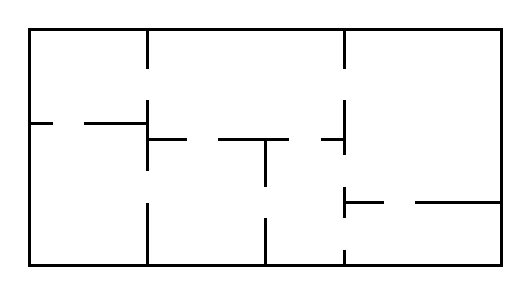
\begin{tikzpicture}
    \draw[very thick] (-3,0) rectangle (3,3);
    \draw[very thick] (-3,1.8) --(-2.7,1.8) (-2.3,1.8) -- (-1.5, 1.8) (-1.5, 1.6) -- (-1,1.6) (-.6, 1.6) -- (.3,1.6) (.7,1.6) -- (1, 1.6) (1, .8) -- (1.5, .8) (1.9,.8) -- (3,.8); 
    \draw[very thick] (-1.5,0) -- (-1.5, .8) (-1.5, 1.2) -- (-1.5,2.1) (-1.5,2.5) -- (-1.5,3);
    \draw[very thick] (0,0) -- (0,.6) (0,1) -- (0,1.6);
    \draw[very thick] (1,0) -- (1,.2) (1,.6) -- (1,1) (1,1.4) -- (1,2.1) (1,2.5) -- (1,3);
  \end{tikzpicture}
\end{center}


\begin{parts}
 \part Edward wants to give a tour of his new pad to a lady-mouse-friend.  Is it possible for them to walk through every doorway exactly once?  If so, in which rooms must they begin and end the tour? Explain.
\part Is it possible to tour the house visiting each room exactly once?  Explain.
\part After a few mouse-years, Edward decides to remodel.  He would like to add some new doors between the rooms he has.  Of course, he cannot add any doors to the exterior of the house.  Is it possible for each room to have an odd number of doors? Explain.
\end{parts}


\question[4] Suppose you are at a party with 19 of your closest friends (so including you, there are 20 people there).  Explain why there must be least two people at the party who are friends with the same number of people at the party.  Assume friendship is always reciprocated.

\question[4] Prove that the {\em Petersen graph} (below) is not planar.  Hint: what is the length of the shortest circuit?

\begin{center}
  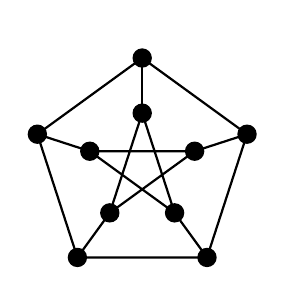
\begin{tikzpicture}[scale=.7]
    \draw[thick] (18:2) -- (90:2) -- (162:2)  -- (234:2) -- (306:2) -- cycle; 
    \draw[thick] (18:1) --  (162:1)  -- (306:1) -- (90:1) -- (234:1) --cycle;
    \foreach \x in {18, 90, 162, 234, 306}
    \draw[thick] (\x:1) \v -- (\x:2) \v;
  \end{tikzpicture}
\end{center}

\question[6] A group of 10 friends decides to head up to a cabin in the woods (where nothing could possibly go wrong).  Unfortunately, a number of these friends have dated each other in the past, and things are still a little awkward.  To get the cabin, they need to divide up into some number of cars, and no two people who dated should be in the same car.
\begin{parts}
  \part What is the smallest number of cars you need if all the relationships were strictly heterosexual?  Represent an example of such a situation with a graph.  What kind of graph do you get?
  \part What is the smallest number of cars you need if the relationships could be represented by the Petersen graph (above)?  Assume each person is represented by a vertex, and two people have dated if there is an edge between their vertices. Explain.
  \part What do these questions have to do with coloring? 
\end{parts}


\end{questions}




\end{document}


